\section{Evaluation and results}
\label{sec:results}
Equipped with \sys, we applied our techniques to nine years of archived Tor
network data, resulting in several megabytes of CSV files and uptime images.  We
sorted our results in descending order by severity, and started manually
analyzing the most significant incidents.  Several outliers were caused by
problems and events in the Tor network that were unrelated to Sybil relays.
Instead of providing an exhaustive list of all potential Sybils, we focus on our
most salient findings---relay groups that were either clearly malicious or
distinguished themselves otherwise.\footnote{Our datasets and visualizations are
available online, and can be inspected for an exhaustive list of potential
Sybils.  The URL is \url{https://nymity.ch/sybilhunting/}.}

Once we discovered a seemingly harmful Sybil group, we reported it to The Tor
Project.  To defend against Sybil attacks, directory authorities can either
remove a relay from the consensus, or take away its \texttt{Valid} flag, which
means that the relay is still in the consensus, but Tor clients will not
consider it for their first or last hop in a circuit.  The majority of directory
authorities, i.e., five out of eight, must agree on either strategy.  This
mechanism is meant to distribute the power of removing relays into the hands of
a diverse set of people.

We present our results by first giving an overview of the most interesting
Sybils we discovered in Section~\ref{sec:sybil_groups}; followed by
technique-specific results in Sections~\ref{sec:churn}, \ref{sec:uptime}, and
\ref{sec:fingerprints}; an evaluation of our nearest-neighbor search in
Section~\ref{sec:accuracy}; and the computational cost of our techniques in
Section~\ref{sec:performance}.

\subsection{Sybil characterization}
\label{sec:sybil_groups}
Table~\ref{tab:sybils} shows the most interesting Sybil groups we identified.
The columns show (\emph{i}) what we believe to be the purpose of the Sybils,
(\emph{ii}) when the Sybil group was at its peak size, (\emph{iii}) the ID we
gave the Sybils, (\emph{iv}), the number of Sybil fingerprints, (\emph{v}) the
analysis techniques that could discover the Sybils, and (\emph{vi}) a short
description.  The analysis techniques are abbreviated as ``E'' (exitmap), ``C''
(Churn), ``U'' (Uptime), ``F'' (Fingerprint), and ``N'' (Neighbor search).  We
now discuss the most insightful incidents in greater detail.

\begin{table*}[ht!]
\small
\centering
\begin{tabularx}{\textwidth}{c|c c c c X}
\hline
\textbf{Purpose} & \textbf{Peak activity} & \textbf{Group ID} & \textbf{Number} &
\textbf{Method} & \textbf{Description} \\
\hline
\multirow{6}{*}{\textbf{MitM}}
& Jan 2016 & rewrite$\dagger$ & 42 & E & Replaced onion domains with
impersonation site. \\

& Nov 2015 & rewrite$\dagger$ & 8 & E & Replaced onion domains with impersonation
site. \\

& Jun 2015 & rewrite$\dagger$ & 55 & E & Replaced onion domains with
impersonation site. \\

& Apr 2015 & rewrite$\dagger$ & 71 & U,E & Replaced onion domains with
impersonation site. \\

& Mar 2015 & redirect$\ddagger$ & 24 & E & Redirected users to impersonated site.
\\

& Feb 2015 & redirect$\ddagger$ & 17 & E & Redirected users to impersonated site.
\\

& Jan 2015 & redirect$\ddagger$ & 26 & E & Redirected users to impersonated site.
\\

\hline

\multirow{2}{*}{\textbf{Botnet}}
& Mar 2014 & default & --- & N & Likely a Windows-powered botnet.  The group
features wide geographical distribution, which is uncommon for typical Tor
relays. \\

& Oct 2010 & trotsky & 649 & N & The relays were likely part of a botnet.  They
appeared gradually, and were all running Windows. \\

\hline

\multirow{5}{*}{\textbf{Unknown}}
& Jan 2016 & cloudvps & 61 & C,U & Hosted by Dutch hoster XL Internet Services. \\

& Nov 2015 & 11BX1371 & 150 & C,U & All relays were in two /24 networks and a single
relay had the \texttt{Exit} flag.  \\

& Jul 2015 & DenkoNet & 58 & U & Hosted on Amazon AWS and only present in a single
consensus.  No relay had the \texttt{Exit} flag. \\

& Jul 2015 & cloudvps & 55 & C,U & All relays only had the \texttt{Running} and
\texttt{Valid} flag.  As their name suggests, the relays were hosted by the
Dutch hoster ``CloudVPS.'' \\

& Dec 2014 & Anonpoke & 284 & C,U & The relays did not have the \texttt{Exit} flag
and were removed from the network before they could get the \texttt{HSDir} flag.
\\

& Dec 2014 & FuslVZTOR & 246 & C,U & The relays showed up only hours after the
LizardNSA incident. \\

\hline

\multirow{1}{*}{\textbf{DoS}}
& Dec 2014 & LizardNSA & 4,615 & C,U & A group publicly claimed to be
responsible for the attack~\cite{lizards}.  All relays were hosted in the Google
cloud and The Tor Project removed them within hours. \\

\hline

\multirow{4}{*}{\textbf{Research}}
& May 2015 & fingerprints & 168 & F & All twelve IP addresses, located in the
same /24, changed their fingerprint regularly, presumably in an attempt to
manipulate the distributed hash table. \\

& Mar 2014 & FDCservers & 264 & C,U & Relays that were involved in an
experimental onion service deanonymization attack~\cite{cmucert}. \\

& Feb 2013 & AmazonEC2 & 1,424 & F,C,U & We observed 1,424 relay fingerprints on
88 IP addresses.  These Sybils were likely part of a research
project~\cite{Biryukov2013a}. \\

& Jun 2010 & planetlab & 595 & C,U & According to a report from The Tor
Project~\cite{progressreport}, a researcher started these relays to learn more
about scalability effects. \\

\hline

\end{tabularx}
\caption{The Sybil groups we discovered using \sys and our exitmap
modules.  We believe that groups marked with the
symbols $\dagger$ and $\ddagger$ were run by the same operator, respectively.}
\label{tab:sybils}
\end{table*}

\paragraph{The ``rewrite'' Sybils}
These recurring Sybils hijacked Bitcoin transactions by rewriting Bitcoin
addresses.  All relays had the \texttt{Exit} flag and replaced onion domains
found in a web server's HTTP response with an impersonation domain, presumably
hosted by the attacker.  Interestingly, the impersonation domains shared a
prefix with the original.  For example, \textbf{sigaint}evyh2rzvw.onion was
replaced with the impersonation domain \textbf{sigaint}z7qjj3val.onion whose
first seven digits are identical to the original.  The attacker could create
shared prefixes by repeatedly generating key pairs until the hash over the
public key resembled the desired prefix.  Onion domains are generated by
determining the SHA-1 hash over the public key, truncating it to its 80 most
significant bits, and encoding it in Base32.  Each Base32 digit of the
16-digit-domain represents five bits.  Therefore, to get an $n$-digit prefix in
the onion domain, $2^{5 n - 1}$ operations are required on average.  For the
seven-digit prefix above, this results in $2^{5 \cdot 7 - 1} = 2^{34}$
operations.  The author of scallion~\cite{scallion}, a tool for generating
vanity onion domains, determined that an nVidia Quadro K2000M, a mid-range
laptop GPU, is able to generate 90 million hashes per second.  On this GPU, a
partial collision for a seven-digit prefix can be found in $2^{34} \cdot
\frac{1}{90,000,000} \simeq 190$ seconds, i.e., just over three minutes.

We inspected some of the phishing domains and found that the attackers replaced
the original Bitcoin addresses, presumably with addresses under their control,
to hijack transactions.  Therefore, we believe that this attack was financially
motivated.

\paragraph{The ``redirect'' Sybils}
These relays all had the \texttt{Exit} flag and tampered with HTTP redirects of
exit traffic.  Some Bitcoin sites would redirect users from their HTTP site to
the encrypted HTTPS version, to protect their users' login credentials.  This
Sybil group tampered with the redirect and directed users to an impersonation
site, resembling the original Bitcoin site, perhaps to steal credentials.  We
only observed this attack for Bitcoin sites, but cannot rule out that other
sites were not attacked.

Interestingly, the Sybils' descriptors and consensus entries had less in common
than other Sybil groups.  They used a small set of different ports, Tor
versions, bandwidth values, and their nicknames did not exhibit an
easily-recognizable pattern.  In fact, the only reason why we know that these
Sybils belong together is because their attack was identical.

We discovered three Sybil groups that implemented the redirect attack, each of
them beginning to surface when the previous one got blocked.  The initial group
first showed up in May 2014, with only two relays, but slowly grew over time,
until it was finally discovered in January 2015.  We believe that these Sybils
were run by the same attacker because their attack was identical.

It is possible that this Sybil group was run by the same attackers that
controlled the ``rewrite'' group but we have no evidence to support that
hypothesis.  Interestingly, only our exitmap module was able to spot these
Sybils.  The relays joined the network gradually over time and had little in
common in their configuration, which is why our \sys methods failed.  In fact,
we cannot rule out that the adversary was upstream, or gained control over these
relays.

\paragraph{The ``FDCservers'' Sybils}
These Sybils were used to deanonymize onion service users, as discussed by The
Tor Project in a July 2014 blog post~\cite{cmucert}.  Supposedly, CMU/CERT
researchers were executing a traffic confirmation attack by sending sequences of
\texttt{RELAY\_EARLY} and \texttt{RELAY} cells as a signal down the circuit to
the client, which the reference implementation never
does~\cite{cmucert,cmucert2}.  The attacking relays were onion service
directories and guards, allowing them to control both ends of the circuit for
some Tor clients that were fetching onion service descriptors.  Most relays were
running FreeBSD, used Tor in version 0.2.4.18-rc, had identical flags, mostly
identical bandwidth values, and were located in 50.7.0.0/16 and 204.45.0.0/16.
All of these shared configuration options made the relays easy to identify.

The relays were added to the network in batches, presumably starting in October
2013.  On January 30, 2014, the attackers added 58 relays to the 63 existing
ones, giving them control over 121 relays.  On July 8, 2014, The Tor Project
blocked all 123 IP addresses that were running at the time.

\paragraph{The ``default'' Sybils}
This group, named after the Sybils' shared nickname ``default,'' has been around
since September 2011 and consists of Windows-powered relays only.  We extracted
relays by filtering consensuses for the nickname ``default,'' onion routing port
443, and directory port 9030.  The group features high IP address churn.  For
October 2015, we found ``default'' relays in 73 countries, with the top three
countries being Germany~(50\%), Russia~(8\%), and Austria~(7\%).  The majority
of these relays, however, has little uptime.
Figure~\ref{fig:default-sybils-uptime} shows the uptime matrix for ``default''
relays in October 2015.  Many relays exhibit a diurnal pattern, suggesting that
they are powered off regularly---as it often is the case for desktop computers
and laptops.

\begin{figure}[t]
	\centering
	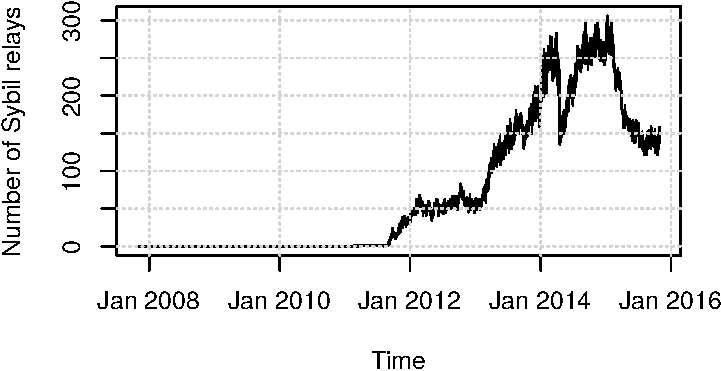
\includegraphics[width=\linewidth]{diagrams/default-over-time}
	\caption{The number of ``default'' and ``trotsky'' Sybil members over time.}
	\label{fig:default-over-time}
\end{figure}

To get a better understanding of the number of ``default'' relays over time, we
analyzed all consensuses, extracting the number of relays whose nickname was
``default,'' whose onion routing port was 443, and whose directory port was
9001.  We did this for the first consensus every day and plot the result in
Figure~\ref{fig:default-over-time}.  Note that we might overestimate the numbers
as our filter could capture unrelated relays.

The above suggests that some of the ``default'' relays are running without the
owner's knowledge.  While the relays do not fit the pattern of Sefnit (a.k.a.
Mevade)~\cite{sefnit} and Skynet~\cite{skynet}---two pieces of malware that use
an onion service as command and control server---we believe that the ``default''
relays constitute a botnet.

\paragraph{The ``trotsky'' Sybils}
Similar to the ``default'' group, the ``trotsky'' relays appear to be part of
a botnet.  Most of the relays' IP addresses were located in Eastern Europe, in
particular in Slovenia, Croatia, and Bosnia and Herzegovina.  The relays were
all running on Windows, in version 0.2.1.26, and listening on port 443.  Most of
the relays were configured as exits, and The Tor Project assigned some of them
the \texttt{BadExit} flag.

The first ``trotsky'' members appeared in September 2010.  Over time, there were
two relay peaks, reaching 139 (September 23) and 219 (October 3) relays, as
illustrated in Figure~\ref{fig:default-over-time}.  After that, only 1--3 relays
remained in the consensus.

\paragraph{The ``Amazon EC2'' Sybils}
The relays all used randomly-generated nicknames, consisting of sixteen or
seventeen letters and numbers; Tor in version 0.2.2.37; GNU/Linux; and IP
addresses in Amazon's EC2 netblock.  Each of the 88 IP addresses changed its
fingerprint 24 times, but not randomly: the fingerprints were chosen
systematically, in a small range.  For example, relay 54.242.248.129 had
fingerprints with the prefixes \texttt{8D}, \texttt{8E}, \texttt{8F}, and
\texttt{90}.  The relays were online for 48 hours.  After 24 hours, most of the
relays obtained the \texttt{HSDir} flag.

We believe that this Sybil group was run by Biryukov, Pustogarov, and Weinmann
as part of their Security and Privacy 2013 paper ``Trawling for Tor Hidden
Services''~\cite{Biryukov2013a}---one of the few Sybil groups that were likely
run by academic researchers.

\paragraph{The ``FuslVZTOR'' Sybils}
All machines were middle relays and hosted in 212.38.181.0/24, which is owned by
a UK VPS provider.  The directory authorities started rejecting the relays five
hours after they joined the network.  The relays advertized the default bandwidth
of 1 GiB/s and used randomly determined ports.  The Sybils were active in
parallel to the ``LizardNSA'' attack, but there is no reason to believe that
both incidents were related.

\paragraph{The ``Anonpoke'' Sybils}
All relays shared the nickname ``Anonpoke'' and were online for four hours until
they were rejected.  All relays were hosted by a VPS provider in the U.S.,
Rackspace, with the curious exception of a single relay that was hosted in the
UK, and running a different Tor version.  The relays advertized the default
bandwidth of 1 GiB/s on port 9001 and 9030.  All relays were middle relays and
running as directory mirror.  All Sybils were configured to be an onion service
directory, but did not manage to get the flag in time.

\paragraph{The ``PlanetLab'' Sybils}
A set of relays that used a variation of the strings ``planet'', ``plab'',
``pl'', and ``planetlab'' as their nickname.  The relays' exit policy allowed
ports 6660--6667, but they did not get the \texttt{Exit} flag.  The Sybils were
online for three days and then removed by The Tor Project, as mentioned in a
blog post~\cite{progressreport}.  The blog post further says that the relays
were run by a researcher to learn more about ``cloud computing and scaling
effects.''

\paragraph{The ``LizardNSA'' Sybils}
All relays were hosted in the Google Cloud and only online for ten hours, until
the directory authorities started to reject them.  The majority of machines were
middle relays (96\%), but the attackers also started some exit relays (4\%).
The Sybils were set up to be onion service directories, but the relays were
taken offline before they could earn the \texttt{HSDir} flag.  If all relays
would have obtained the \texttt{HSDir} flag in time, they would have constituted
almost 50\% of all onion service directories; the median number of onion
service directories on December 26 was 3,551.

Shortly after the attack began, somebody claimed responsibility on the tor-talk
mailing list~\cite{lizards}.  Judging by the supposed attacker's demeanor, the
attack was mere mischief.

\subsection{Churn rate analysis}
\label{sec:churn}
We determined the churn rate between two subsequent consensuses for all 72,061
consensuses that were published between October 2007 and January 2016.
Considering that (\emph{i}) there are 162 gaps in the archived data, that
(\emph{ii}) we create time series for joining and leaving relays, and that
(\emph{iii}) we determined churn values for all twelve relay flags, we ended up
with $(72,061 - 162) \cdot 2 \cdot 12 = 1,725,576$ churn values.
Figure~\ref{fig:churn-boxplot} shows a box plot for the churn distribution
(joining and leaving churn values concatenated) for the seven most relevant
relay flags.  We removed values greater than the plot whiskers (which extend to
values $1.5$ times the interquartile range from the box) to better visualize the
width of the distributions.  Unsurprisingly, relays with the \texttt{Guard},
\texttt{HSDir}, and \texttt{Stable} flag experience the least churn, probably
because relays are only awarded these flags if they are particularly stable.
Exit relays have the most churn, which is surprising given that exit relays are
particularly sensitive to operate.  Interestingly, the median churn rate of the
network has steadily decreased over the years, from $0.04$ in 2008 to $0.02$ in
2015.

\begin{figure}[t]
	\centering
	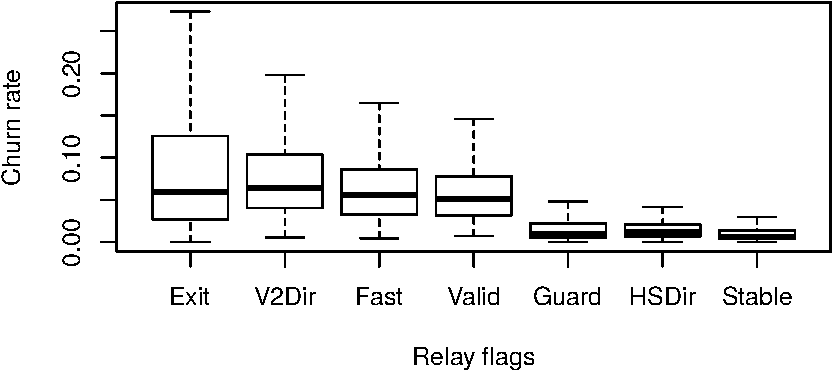
\includegraphics[width=\linewidth]{diagrams/churn-boxplot.pdf}
	\caption{The churn distribution for seven relay flags.  We removed values
		greater than the plot whiskers.}
	\label{fig:churn-boxplot}
\end{figure}

Figure~\ref{fig:2008-08} illustrates churn rates for five days in August 2008,
featuring the most significant anomaly in our data.  On August 19, 822 relays
left the network, resulting in a sudden spike, and an increase in the baseline.
The spike was caused by the Tor network's switch from consensus format version
three to four.  The changelog says that in version four, routers that
do not have the \texttt{Running} flag are no longer listed in the consensus.

\begin{figure}[t]
	\centering
	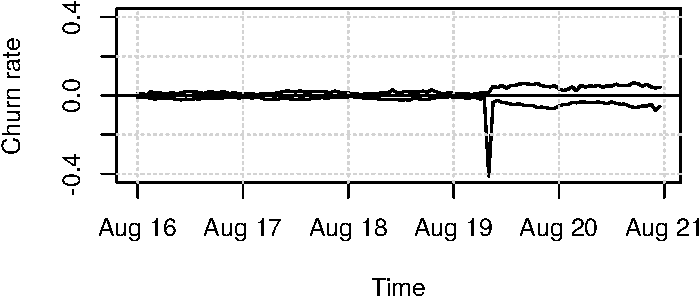
\includegraphics[width=\linewidth]{diagrams/2008-08.pdf}
	\caption{In August 2008, an upgrade in Tor's consensus format caused the
	biggest anomaly in our dataset.  The positive time series represents relays
	that joined and the negative one represents relays that left.}
	\label{fig:2008-08}
\end{figure}

To alleviate the choice of a detection threshold, we plot the number of alerts
(in log scale) in 2015 as the threshold increases.  We calculate these numbers
for four simple moving average window sizes.  The result is shown in
Figure~\ref{fig:threshold-alarm}.  Depending on the window size, thresholds
greater than 0.012 seem practical considering that 181 alerts per year average
to approximately one alert in two days---a tolerable number of incidents to
investigate.  Unfortunately, we are unable to determine the false positive rate
because we do not have ground truth.

\begin{figure}[t]
	\centering
	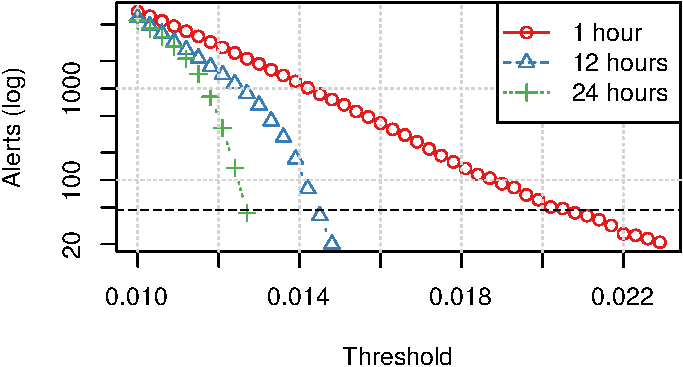
\includegraphics[width=0.9\linewidth]{diagrams/threshold-alarm.pdf}
	\caption{The number of alerts (in log scale) in 2015 as the detection
	threshold increases, for three smoothing window sizes.}
	\label{fig:threshold-alarm}
\end{figure}

\subsection{Uptime analysis}
\label{sec:uptime}
We generated relay uptime visualizations for each month since 2007, resulting in
100 images.  We now discuss a subset of these images that contain particularly
interesting patterns.

Figure~\ref{fig:2010-06-planetlab} shows June 2010, featuring a clear ``Sybil
block'' on the left side.  The Sybils belonged to a researcher who, as
documented by The Tor Project~\cite{progressreport}, started several hundred Tor
relays on PlanetLab for research on scalability.  Our manual analysis could
verify this.  The relays were easy to identify because their nicknames suggested
that they were hosted on PlanetLab, containing strings such as ``planetlab,''
``planet,'' and ``plab.''  Note the small height of the Sybil block, indicating
that the relays were only online for a short time.

\begin{figure}[t]
	\centering
	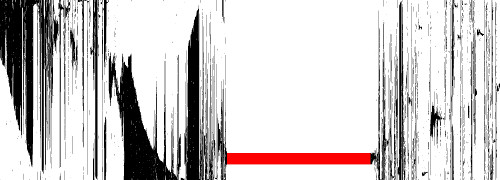
\includegraphics[width=\linewidth]{diagrams/2010-06.jpg}
	\caption{In June 2010, a researcher started several hundred Tor relays on
		PlanetLab~\cite{progressreport}.  Die image shows the uptime of 2,000
		relays for all of June.}
	\label{fig:2010-06-planetlab}
\end{figure}

Figure~\ref{fig:2012-08-steppattern} features a curious ``step pattern'' for
approximately 100 relays, all of which were located in Russia and Germany.  The
relays appeared in December 2011, and started exhibiting the diurnal step
pattern (nine hours uptime followed by fifteen hours downtime) in March 2012.
All relays had similar nicknames, consisting of eight seemingly
randomly-generated characters.  In April 2013, the relays finally disappeared.

\begin{figure}[t]
	\centering
	
\includegraphics[width=\linewidth]{diagrams/2012-08.jpg}
	\caption{August 2012 featured a curious ``step pattern,'' caused by
	approximately 100 Sybils.  The image shows the uptime of 2,000 relays for
	all of August.}
	\label{fig:2012-08-steppattern}
\end{figure}

Figure~\ref{fig:2014-04-heartbleed} shows the effect of the Heartbleed
incident~\cite{Durumeric2014a} on the Tor network.  Several days after the
incident, The Tor Project decided to block all relays that had not generated new
key pairs.  The large red rectangle on the left side of the image illustrates
when the biggest part of the block became active, rejecting approximately 1,700
Tor relay fingerprints.
% $ wc -l dirauth-conf/approved-routers.d/bleeding-edges.conf
% 1779 dirauth-conf/approved-routers.d/bleeding-edges.conf

\begin{figure}[t]
	\centering
	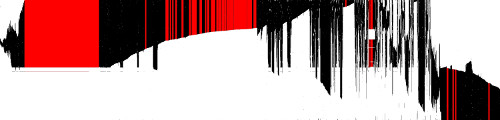
\includegraphics[width=\linewidth]{diagrams/2014-04.jpg}
	\caption{In April 2014, the Heartbleed bug forced The Tor Project to reject
	many affected relays.  The image shows the uptime of 3,000 relays for all of
	April.}
	\label{fig:2014-04-heartbleed}
\end{figure}

Figure~\ref{fig:2014-12-lizard} illustrates the largest Sybil group to date,
comprising 4,615 Tor relays that an attacker started in the Google cloud in
December 2014.  Because of its magnitude, the attack was spotted almost
instantly, and The Tor Project removed the offending relays only ten hours
after they appeared.

\begin{figure}[t]
	\centering
	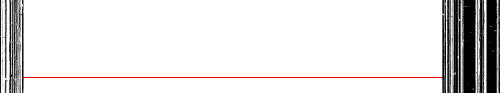
\includegraphics[width=\linewidth]{diagrams/2014-12.jpg}
	\caption{In December 2014, a group of attacker started several hundred Tor
		relays in the Google cloud.  The image shows the uptime of 4,000 relays
		for all of December.}
	\label{fig:2014-12-lizard}
\end{figure}

\subsection{Fingerprint anomalies}
\label{sec:fingerprints}
We determined how often all Tor relays changed their fingerprint from 2007 to
2015.  Figure~\ref{fig:fingerprints} illustrates the number of fingerprints ($y$
axis) we have observed for the 1,000 Tor relays ($x$ axis) that changed their
fingerprint the most.  All these relays changed their fingerprint at least ten
times.  Twenty one relays changed their fingerprint more than 100 times, and the
relay at the very right end of the distribution changed its fingerprint 936
times.  This relay's nickname was ``openwrt,'' suggesting that it was a home
router that was rebooted regularly.  It was running from August 2010 to December
2010.

\begin{figure}[t]
	\centering
	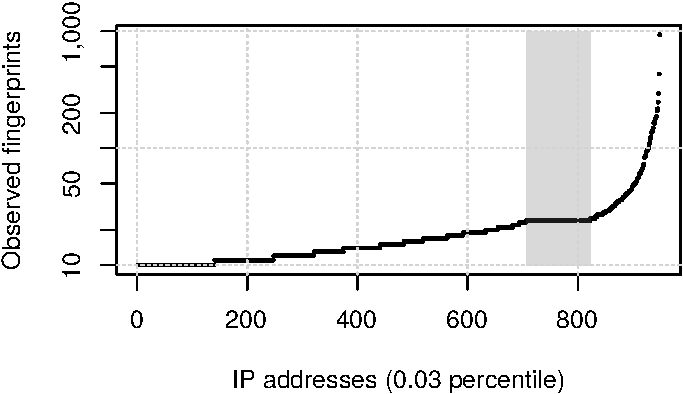
\includegraphics[width=0.9\linewidth]{diagrams/fingerprints.pdf}
	\caption{The number of observed fingerprints for the 1,000 relays that
	changed their fingerprints the most.}
	\label{fig:fingerprints}
\end{figure}

Figure~\ref{fig:fingerprints} further contains a peculiar plateau, shown in the
shaded area between index 707 and 803.  This plateau was caused by a group of
Sybils, hosted in Amazon EC2, that changed their fingerprint exactly 24 times.
Upon inspection, we noticed that this was likely an experiment for a Security
and Privacy 2013 paper on deanonymizing Tor onion services~\cite{Biryukov2013a}.

We also found that many IP addresses in the range 199.254.238.0/24 changed their
fingerprint frequently.  We contacted the owner of the address block and were
told that the block used to host VPN services.  Apparently, several people
started Tor relays and since the VPN service would not assign permanent IP
addresses, the Tor relays would periodically change their address, causing the
churn we observe.

\subsection{Accuracy of nearest-neighbor search}
\label{sec:accuracy}
Given a single Sybil relay, how good is our nearest-neighbor search at finding
the remaining Sybils?  To answer this question, we now evaluate our algorithm's
\emph{accuracy}, which we define as the fraction of neighbors it correctly
labels as Sybils.  For example, if eight out of ten Sybils are correctly labeled
as neighbors, the accuracy is 0.8.

A sound evaluation requires ground truth, i.e., relays that are \emph{known} to
be Sybils.  All we have, however, are relays that we \emph{believe} to be
Sybils.  In addition, the number of Sybils we found is only a lower bound---we
are unlikely to have detected all Sybil groups.  Therefore, our evaluation is
doomed to overestimate our algorithm's accuracy because we are unable to test it
on the Sybils we did not discover.

We evaluate our search algorithm on two datasets; the ``bad exit'' Sybil groups
from Table~\ref{tab:exitmap-dataset}, and relay families.  We chose the bad exit
Sybils because we observed them running identical, active attacks, which makes
us confident that they are in fact Sybils.  Recall that a relay family is a set
of Tor relays that is controlled by a single operator, but configured to express
this mutual relationship in the family members' configuration file.  Relay
families are benign Sybils.  As of January 2016, approximately 400 families
populate the Tor network, ranging in size from only two to 25 relays.

We evaluate our algorithm by finding the nearest neighbors of a family member.
Ideally, all neighbors are family members, but the use of relay families as
ground truth is very likely to overestimate results because family operators
frequently configure their relays identically on purpose.  At the time of this
writing, a popular relay family has the nicknames ``AccessNow000'' to
``AccessNow009,'' adjacent IP addresses, and identical contact
information---perfect prerequisites for our algorithm.  We expect the operators
of malicious Sybils, however, to go out of their way to obscure the relationship
between their relays.

To determine our algorithm's accuracy, we used all relay families that were
present in the first consensus that was published in October 2015.  For each
relay that had at least one mutual family relationship, we searched for its $n -
1$ nearest neighbors where $n$ is the family size.  Basically, we evaluated how
good our algorithm is at finding the relatives of a family member.  We
determined the accuracy---a value in $[0,1]$---for each family member.  The
result is shown in Figure~\ref{fig:family-accuracy}, a distribution of accuracy
values.

Next, we repeated the evaluation with the bad exit Sybil groups from
Table~\ref{tab:exitmap-dataset}.  Again, we searched for the $n - 1$ nearest
neighbors of all bad exit relays, where $n$ is the size of the Sybil group.  The
accuracy is the fraction of relays that our algorithm correctly classified as
neighbor.  The result is illustrated in Figure~\ref{fig:badexit-accuracy}.

\begin{figure}
\centering
\subfigure[Bad exit relay Sybils]{
	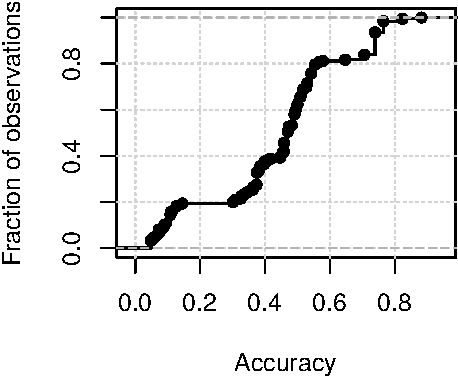
\includegraphics[width=0.46\linewidth]{diagrams/bad-relay-accuracy.pdf}
\label{fig:badexit-accuracy}
}
\subfigure[Benign family Sybils]{
	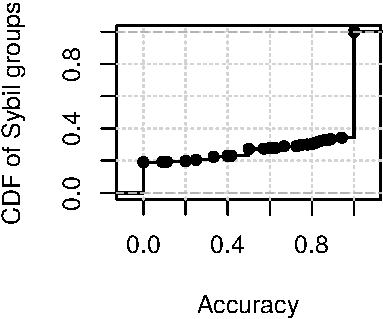
\includegraphics[width=0.46\linewidth]{diagrams/family-accuracy.pdf}
\label{fig:family-accuracy}
}
\caption{ECDF for our two evaluations, the bad exit Sybils
	in Fig.~\ref{fig:badexit-accuracy} and the benign family Sybils
	in Fig.~\ref{fig:family-accuracy}.}
\label{fig:accuracy}
\end{figure}

As expected, our algorithm is significantly more accurate for the family
dataset---66\% of searches had perfect accuracy.  The bad exit dataset, however,
did worse.  Not a single search had perfect accuracy and 59\% of all searches
had an accuracy in the interval $[0.3,0.6]$.  Nevertheless, we find that our
search algorithm facilitates manual analysis given how quickly it can provide us
with a list of the most similar relays.  Besides, false positives (i.e.,
neighbors that are not Sybils) are cheap as \sys users would not spend much time
on neighbors that bear little resemblance to the ``seed'' relay.

\subsection{Computational cost}
\label{sec:performance}
Fast techniques lend themselves to being run hourly, for every new consensus,
while slower ones must be run less frequent.  Table~\ref{tab:exp-deployment}
gives an overview of the runtime of our methods.\footnote{We determined all
performance numbers on an Intel Core i7-3520M CPU at 2.9 GHz, a consumer-grade
CPU.}  We stored our datasets on a solid state drive to eliminate I/O as
performance bottleneck.

\begin{table}[t]
	\centering
	\begin{tabular}{lcc}
	\hline
	\textbf{Method} & \textbf{Analysis window} & \textbf{Run time} \\
	\hline
	Churn & Two consensuses & $\sim$0.16s \\
	Neighbor search & One consensus & $\sim$1.6s \\
	Fingerprint & One month & $\sim$58s \\
	Uptimes & One month & $\sim$145s \\
	\hline
	\end{tabular}
	\caption{The computational cost of our analysis techniques.}
	\label{tab:exp-deployment}
\end{table}

The table columns contain, from left to right, our analysis technique, the
technique's analysis window, and how long it takes to compute its output.
Network churn calculation is very fast; it takes as input only two consensus
files and can easily be run for every new network consensus.  Nearest-neighbor
search takes approximately 1.6 seconds for a single consensus counting 6,942
relays.  Fingerprint and uptime analysis for one month worth of consensuses
takes approximately one and two minutes, respectively---easy to invoke daily, or
even several times a day.
